\documentclass[10pt,a4paper]{article}
\usepackage[utf8]{inputenc}
\usepackage[scale=0.7,vmarginratio={1:2},heightrounded]{geometry}

\usepackage{multicol}
\setlength{\columnsep}{1cm}
\usepackage{scrextend}
\addtokomafont{labelinglabel}{\sffamily}
\usepackage[numbers]{natbib}

\usepackage[strings]{underscore}

% inline enumeration
\usepackage{enumitem}

\newlist{inlinelist}{enumerate*}{1}
\setlist*[inlinelist,1]{%
  label=(\roman*),
}

% link support in pdf
\usepackage[colorlinks,allcolors=blue,breaklinks = true]{hyperref}

% images in pdf
\usepackage{graphicx}
\graphicspath{{Images/}}
% multiple images
\usepackage{subfigure}
% images float in text
\usepackage{float}

% url support
\usepackage{url}
% glossarie support
\usepackage[acronym, automake]{glossaries}
\makeglossaries
\loadglsentries{myGlossary}

% math libs
\usepackage{amsmath}
\usepackage{amssymb}
\usepackage{amstext}
\usepackage{amsfonts}
\usepackage{mathrsfs}

% Code formating
\usepackage{listings}
\usepackage{color}

% subfile to include titlepage. Possible to gitignore titlepage with private information
\usepackage{subfiles}

\definecolor{dkgreen}{rgb}{0,0.6,0}
\definecolor{gray}{rgb}{0.5,0.5,0.5}
\definecolor{mauve}{rgb}{0.58,0,0.82}

\lstset{frame=tb,
  language=Java,
  aboveskip=3mm,
  belowskip=3mm,
  showstringspaces=false,
  columns=flexible,
  basicstyle={\small\ttfamily},
  numbers=none,
  numberstyle=\tiny\color{gray},
  keywordstyle=\color{blue},
  commentstyle=\color{dkgreen},
  stringstyle=\color{mauve},
  breaklines=true,
  breakatwhitespace=true,
  tabsize=3
}

%Metadata
\title{Procedural Generation in tools}
\author{Simon Hischier}
\date{April 2019}

\begin{document}

\subfile{titlepageReal}


%Table of Contents Page
\renewcommand{\contentsname}{Content}
\tableofcontents
\newpage

%First real page
\section{Abstract}
\label{sec:abstract}
\begin{multicols}{2}
This work discusses the relation between the past lack of procedural content generation in the game industry with the recent uptake of procedural content generation in emerging tools for game developers and artists and the use of procedural content generation in the game industry. How is procedural content generation as part of games and as a developing tool changing so that it is gaining relevance in the games industry and related sectors? New tools and a more data-driven approach to procedural content generation in recent years have lead to a less noticeable but steady increase in usage across a number of disciplines and workfields and a shift in toolsets in the game industry. The paper observes and analyzes the trends and explains the newfound interest through analogy, literature review, market and workflow analysis. We highlight the deviating techniques these new tools use and where they differ from classic tools based on this we draw a conclusion why procedural content generation gains popularity.
\end{multicols}

\section{Introduction}\label{sec:Introduction}
\begin{multicols}{2}
The cost to make games seems to be on an exponential curve as Raph Koster states in 2018. He suggests among other things that game developers should focus a lot more on algorithmic and procedural approaches to keep the cost of games under control\cite{Koster2018}. On Quora, an online discussion forum, Steve Theodore who worked on \textit{Half-Life} (Valve Corporation, 1998) and other games, explains in which fields artists spend more time and therefore more money. Theodore states, that most extra time is spent on texturing, shading and animation. We find that these are fields where \gls{pcg} has seen huge improvements. He based his reasoning on a practical comparison between two models he worked on. A character model for the game \textit{Half-Life} took about 2 working weeks and a model 10 years later for a different game took him seven working weeks\cite{Prinke2017}.

Increased worktimes and a trend to bigger, more realistic worlds in AAA games is a big problem. Studios developing AAA games have to spend a lot more money to create these resources. In the paper “\textit{The Role of Semantics in Games and Simulations}” Tim Tutenel and Farael Bidarra explain that studios have an ever-increasing pressure to create more models with more realistic looks and behaviour. The big problem the gaming and simulation industry is facing is how the models for these worlds are made. Tim Tutenel et al. in 2008 point out that the models get more complex but how they are made still resembles a high-tech variation on how handicrafts are made\cite{Tutenel2008}. Worlds increase but the amount of time and money that a company can spend on game development is limited. Modern models are only improving in looks but not in semantics\cite{Tutenel2008}. Ultimately new 3D models in games differ mostly in vertex count and how they are rendered. Enhancing new models with additional semantics has the potential to greatly increase the production value of models. Tim Tutenel et al. are using the Wikipedia definition of semantic as related to meaning, significant and to signify, to indicate\cite{Wikipediacontributors2019, Tutenel2008}. Better tools and semantically enhanced models have the potential for rule based world generation where virtually every object is interactable. Models with more semantic information can not only help during the development phase: Games like \textit{The Legend of Zelda: Breath of the Wild} (Nintendo Entertainment Planning \& Development, 2017) show how a basic semantically enhanced world leads to an exponential rise in interactability and a more believable world. Samuel Rantaeskola in 2017 states that in the past systems were less powerful and therefore the limiting factor was optimization. Nowadays the content and its increasing complexity is the big limitation\cite{Prinke2017}. More people working on a project increases overhead and the more work on a project the less impact there is when a single person is added to a team.
Ever-increasing cost of development does come with financial side effects. A lot of big studios closed down or had massive layoffs over the past year \cite{Lahti2018, Schreier2019, Walker2019, Schreier2019a} and this seems to be a long term trend backed by older numbers\cite{Plunkett2012}. The race to higher costs leave midsize studios in an awkward position. They are too big to survive by creating small games but not big enough to compete with AAA games. Steve Theodore recalls seeing a lot of midsize studios closing down in the Seattle area because they grew into big studios, went indie or died\cite{Prinke2017}. As more AAA games get produced, studios not only compete against each other and have to overshadow their own previous work. For artists to keep up with the ever increasing demand for more output in a fixed timeframe, industry software is incorporating \gls{pcg} into their products. \gls{pcg} here seems to be a very promising route. We define \gls{pcg} as a way to generate (game) content through algorithms. It’s a way to automatically generate content and can greatly reduce the workload of artists.
\end{multicols}
\section{Problem/Research Question}
\begin{multicols}{2}
The computer game industry is a rather collaborative and open industry. Knowledge and creative techniques are quickly shared and adapted in different studios. However, the industry is very competitive. Games cost a lot of money and are produced over several years without earning a dollar during the development period. The spent money needs to be reclaimed on game release putting the studios under great pressure. Games are widely different and getting the development cost back is in no way guaranteed. The fact that in developed countries the game markets are close to saturation\cite{Koster2018} does not help. For game studios this results in increased competition with each other. As part of the entertainment industry, games try to have unique features which can be marketed as unique selling points. Each gameseries has its strengths, long running series try to vary the gameplay and, if possible, keeping their core gameplay formula untouched. To achieve this each studio is developing unique workflows, engines, management strategies etc. allowing the studio to stand apart from other studios. This leads to several problems: \begin{inlinelist} \item The production pipeline in each studio is different. Every game engine needs data in different formats sometimes uniquely crafted just for the engine.  \item Acquiring new talents costs a lot of money. Every new employee must learn the engine requirements and how to produce content aimed to meet the engines needs. This difference in engines is one of many reasons why standards for various data formats are minimal. Although Unity and Unreal Engine have helped streamline the workflow for studios in some ways: Some rendering pipelines like the physical based rendering pipeline become widespread and is used on many devices. As an example there is a new 3D object data format called \textit{glTF2.0} to exchange 3D data with textures for physical based rendering as a requirement\cite{TheKhronosGroup}. This helps keeping track of files and reduces checks to load new models. Most engines can use the same texture components (basecolor, metallic, roughness). \item But unique game aspects demand for unique data formats on top of these commonly shared data or need additional information. \item However the dataformats can not help produce content more quickly. The demand for more content in the same timespan remains unsolved with or without common components. Standardized engines did not solve the problem of limited content output\cite{Koster2018}.\end{inlinelist}

This paper gathers several advancements on various fields who are partly responsible why emerging tools differ from traditional solutions. With this tools more \gls{pcg} is integrated in the various steps of game development and the new tools are adapted into workflows slowly but steadily. These new tools yield potential for studios to accelerate workflows and content output. Besides directly influencing productivity, these standardized tools independent from game engines have the potential to immensely reduce the time for new employees to be productive. We base this assumption on several reasons: Independent and widely used tools can be taught in schools. Tools used in different domains greatly reduce the barrier for new talents to enter the gaming industry. In return the developers for this tools profit from a big user base that will grow the community around those tools and can help improve the user experience. A big community increases productivity as more questions are answered and creative people can rely on an increasing knowledge database. With new tools and formats becoming standardized and tested, mainstream engines start to adapt these tools as proven by the adaption of the \textit{glTF2.0} 3D format\cite{Group2018}. A more hidden facette of emerging tools such as \textit{Houdini} (SideFX), \textit{Substance Designer} (Allegorithmic) and \textit{Blender} (Blender Foundation) is, that they all integrate some level of \gls{pcg}. We specifically chose these 3 tools to cover a broad aspect of game development such as pre-production and content generation, modeling and texturing. We chose \textit{Substance Designer} because it is very relevant in the game industry. Alternatives like \textit{NeoTextureEdit} (Holger Dammertz, GNU LGPL v. 3) and \textit{MapZone} (Allegorithmic) are discontinued. \textit{Blender} is a free alternative to \textit{Cinema4D} (Maxon) and \textit{Maya} (Autodesk) with a huge innovative community. \textit{Houdini} is relevant because of the procedural workflow and unique integration in game engines. As pointed out in \autoref{sec:Introduction}, current 3D assets still lack semantics which can be a very powerful katalysator to increase content output. With \gls{pcg} becoming commonplace in tools, the additional work to integrate semantics into content production is greatly reduced. As \gls{pcg} is a core part of this trend we ask the question: How is procedural content generation as part of games and as a developing tool changing so that it is gaining relevance in the games industry and related sectors? \gls{pcg} lets designers iterate on models for previous games and enhancing the data becomes easier. Maturing and tested formats reduce the complexity of the internal engine logic, outsourcing the reading and writing of these formats to middleware converters.
\end{multicols}
\section{Categories of Procedural Generation}\label{sec:categories}
\begin{multicols}{2}
We are using \gls{pcg} categories based on the book \textit{Procedural Generation in Game Design}\citep[p.~3]{Short:2017:PGG:3161477} where the following four categories are described. We chose these categories because it honors the broader game development pipeline. The categorization allows to categorize \gls{pcg} based on where in the production pipeline it’s used and does not categorize what kind of \gls{pcg} is used.
\end{multicols}
\subsection{Integral}
\begin{multicols}{2} The use of \gls{pcg} must be planed and considered in the concept and game design from the get-go. These games rely heavily on a working \gls{pcg} and even core gameplay can be affected. Games such as \textit{Rogue} (A.I. Design, 1980) or a more modern game like \textit{Dwarf Fortress} (Bay 12 Games, 2006) are using \gls{pcg} extensively and would not work without it. They need it to be the type of game they are. Changes to the project planning have vast implications on the codebase. These games are built around central algorithms and project changes will result in redrafting these algorithms.
\end{multicols}
\subsection{Drafting Content}
\begin{multicols}{2} From a game design perspective these games do not rely on \gls{pcg} from the start. Game designers rely on \gls{pcg} to generate initial drafts of game content such as the map or items. These drafts can be looked through by humans and are then handpicked. But before algorithmically generating this initial drafts of the final game content, artists can prototype game parts and handbuild parts to get a better understanding of what the algorithm should generate and to start working on other parts of the game right away. Some games use this method to generate a world which is then polished by humans. An example of generating and polishing is \textit{Skyrim} (Bethesda Game Studios, 2011) and a more recent and sophisticated example is \textit{Far Cry 5} (Ubisoft, 2018) where Carrier Étienne explains how the world was modified by humans but regenerated daily by his team\cite{Carrier2018}.
\end{multicols}
\subsection{Modal}
\begin{multicols}{2} Some games are build with little or even without the use for \gls{pcg} and it gets added later on during development. Even after release, \gls{pcg} can be added in the form of an “infinity mode” or as procedural maps, for example in \textit{Rust} (Facepunch Studios Ltd, 2013). While this type can add a lot of replay value to a game it is mostly used just for that and does not add new or innovative content to the game.
\end{multicols}
\subsection{Segmented}
\begin{multicols}{2} A game where the gameplay, levels, music etc. can be split into independent parts. Some of these parts can include \gls{pcg}. The development can continue with or without these areas. If the desired standard is not met by the algorithm, the team can simply revert to handcrafted content for these areas. The term “areas” does not need to be restricted to levels. It can include parts of the game such as procedural music, graphical effects or randomized elements. At all times, the game developers have the possibility to revert to hand-generated content.
\end{multicols}
\section{Tools for Procedural Content Generation}
\begin{multicols}{2}
At the 2018 Blender Conference in Amsterdam at the Blender HQ, Andrew Price tried to predict changes to the 3D industry in the next 5 to 10 years. A big point besides machine learning assistance becoming a standard is the adaption of procedural workflows and the workflows becoming mainstream\cite{Price2018}. Price states that procedural texturing made by \textit{Substance Designer} in combination with \textit{Substance Painter} (Allegorithmic) is saving big studios money in the range of hundreds of thousands of US Dollars. He elaborates on this by giving an example. His service \textit{Poliigon} (CGFort Pty Ltd) started out photographing real materials but switched to a more labor intensive workflow. Materials are created virtually in \textit{Substance Designer} which comes with a great increase in value: Using these generated materials allows the user to adjust color, add details, scale to infinity and enhance with more semantic information which could then be used for \gls{pcg} or directly in the game engine. We find that \textit{Houdini} is another tool with similar far-reaching consequences. Anastasia Opara in 2017 built a swamp village generator with this tool. The village is completely generated with \gls{pcg} and can generate an endless number of houses. She describes the interesting part of this method is the exploration of what the algorithm creates based on the rules given. “One of the most satisfying part was, when generating the final lake houses, the network would give me unexpected, but very creative results [...]”\cite{Opara2016}. Anastasia Opara sees art as something we can translate into computer language. However, she explains that the workflow was very labor intensive and quite challenging. The village generator was generated in various steps with increasing granularity. As her motivation for this project she states: “My goal was to expand the limits of what is expected from a procedural content generation [...]”\cite{Opara2017}.
\end{multicols}
\section{Procedural Stochastic Textures}
\begin{multicols}{2}
Textures are traditionally a big topic in game development. A lot of research went into textures because it’s a big part of modern rendering pipelines and reaches back to the early days of modern computer graphics. Games in the 80’s and 90’s had hard limits on disk space\cite{Ferrari2016} and designing games involved balancing storage space between program code, music and images. We list two examples on these limitations: Besides a single digital sample channel, sounds on home consoles like the \gls{nes} were limited to hardware generated tones\cite{wiki:NintendoEntertainmentSystem}. Game developers had to generate most of the music via \gls{pcg}. Another limitation was that consoles like the \gls{nes} and \gls{snes} had no chips to calculate complex 3D objects. The Picture Processing unit was used to display only sprites. To fill a TV screen the \gls{nes} and \gls{snes} used texture tiling, a technique for creating small texture samples which can be tiled to create a seamless pattern. This technique is still in use for modern games with more complex textures and increased texture size. Games using \gls{pcg} as an integral part rely heavily on tileable textures or alternatively use generated procedural textures for example Perlin\cite{perlin1985image} or Worley\cite{worley1996cellular} noise. Those approaches come with disadvantages: Tiles are very repetitive and Perlin noise needs very sophisticated algorithms to generate interesting levels. We see a great increase in production value by using another texture generating solution as a modern alternative: By-example noise algorithms. These algorithms take a stochastic example texture and generate larger versions out of it. Until now these were too slow for real time generation and therefore were only suitable for drafting content. A recent paper by Heitz and Neyret created an algorithm able to create stochastic textures on-the-fly\cite{Heitz2018}. This enables artists to build levels and getting direct feedback with final textures already applied during building. This technique even allows for algorithmic level generation without using tile based textures. This is especially important because previously, textures not based on tiles lead to hard edges and repeating patterns shown in \autoref{fig:procStocTexturing}.
\end{multicols}

\begin{figure}[H]
   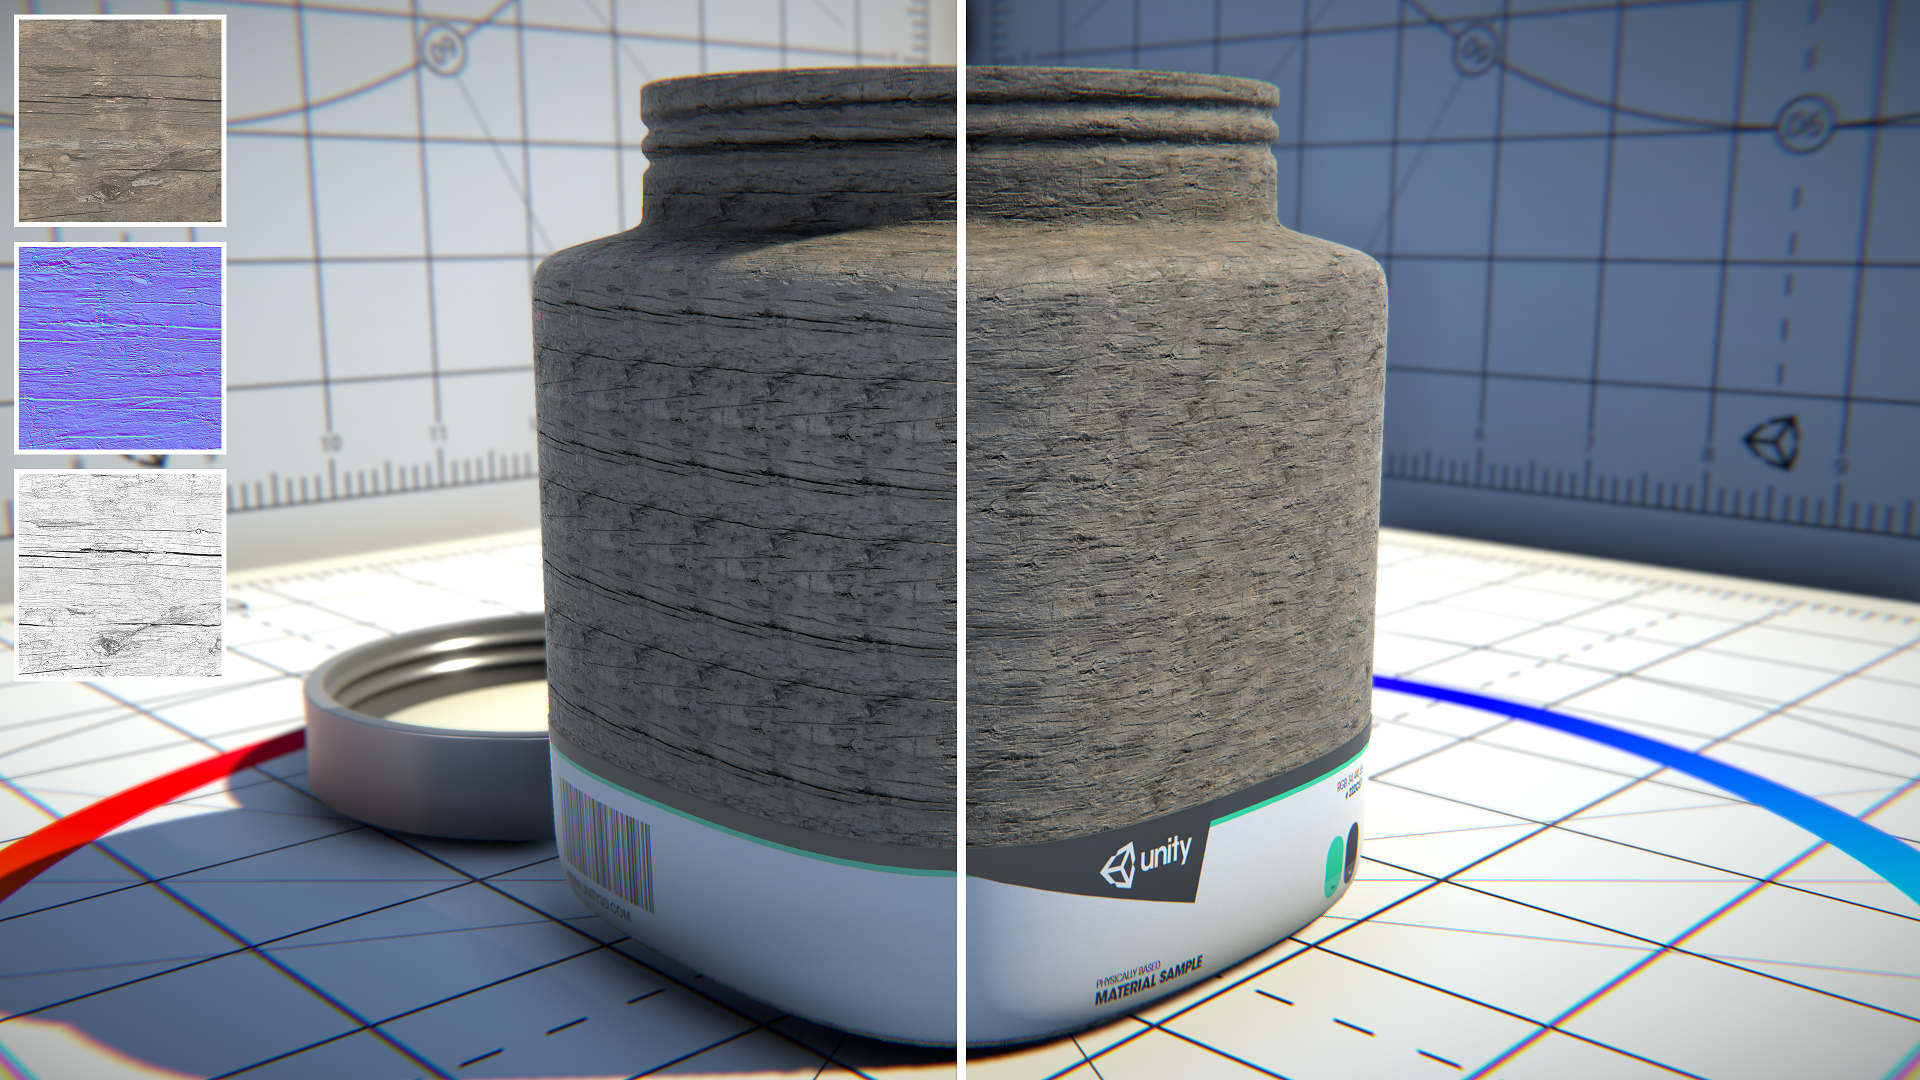
\includegraphics[width=\textwidth, height=\textheight, keepaspectratio]{proceduralStochasticTexturingInUnityExample.png}
   \caption{Wood detail maps with albedo, normal and occlusion textures. Retrieved 11:50, March 9, 2019 from {https://blogs.unity3d.com/2019/02/14/procedural-stochastic-texturing-in-unity/}}
   \label{fig:procStocTexturing}
\end{figure}
\section{WaveFunctionCollapse}\label{sec:WaveFunctionCollapse}
\begin{multicols}{2}
Creating completely new tools for \gls{pcg} is a huge time investment. Darren Grey writes, that using \gls{pcg} is a bad idea when there is a time restriction\citep[p.~6]{Short:2017:PGG:3161477}. It is even worse if \gls{pcg} is used as an integral part of the game. The game stands and falls with the algorithm, every part of the game is influenced by the generation. As an alternative to this high risks we see procedural middleware or usable parts already developed by other companies. An example of a widely used \gls{pcg} algorithm middleware for game studios is SpeedTree\cite{SpeedTree}. The software generates trees for games in all forms and sizes. For a game studio this is a very small investment compared to writing their own tree generator (or even worse, handcrafting) just to fill the background of a scene. However, these kind of software middlewares are scares. Writing a tool in house comes with a lot of additional work. The software should not only generate content, it should be easily understandable, controllable and fast to allow the artists to experiment with it and put the tool to good use. The commercial lack of use of \gls{pcg} algorithms correlates with the lack of their control as Roland van der Linden assumes\cite{VanderLinden2014}. Easy to use tools and algorithms encourage experimentation and leads to faster adaptation of \gls{pcg} techniques as Adam M. Smith shows\cite{Karth2017}. The algorithm called “WaveFunctionCollapse” described by Alexei A. Efros and Thomas K. Leung is very easy to use without programming knowledge\cite{Efros1999}. The algorithm needs an input image and can generate infinitely large output textures. The underlying algorithm works out of the box and does not need tweaking to get great results. This data driven algorithm can be adapted to 3 dimensional space. Oskar Stalberg explains how the islands in the game \textit{Bad North} (Plausible Concept, 2018) are generated by using WaveFunctionCollapse. A more recent tech demo shows infinite city generation with interesting buildings made by only using around 100 building blocks\cite{Marian2019}.
\end{multicols}
\section{Rise of Scripting languages}
\begin{multicols}{2}
John K. Ousterhout wrote a paper\cite{Ousterhout1998} in 1998 where he analyzed the difference in use of system languages (C, C++, Java) and scripting languages (Python, Perl, Javascript). His analysis is important because in this paper we look at visual \gls{ns}s (a part of the dataflow programming paradigm\cite{wiki:Dataflow}) as comparable to scripting languages. He pointed out, that scripting languages are much better suited for casual programmers based on several reasons. One reason is the size of programs. Scripting languages need less lines of code to get the same work done. Higher-level languages need several months of learning to master where as scripting languages lead to results in hours. This is of great importance, it allows a team to hire technical artists who are quickly ready to work on projects. However both languages are required, they are complementary.\begin{quote}
“Scripting languages assume that a collection of useful components already exists in other languages.”\citep[p.~2]{Ousterhout1998}
\end{quote}
The limiting factor in larger adaptations are the power of computers. The paper finds that, the faster computers get the larger the applications built with scripting languages will be. Current developments on various applications indicate that computers are powerful enough for meaningful applications to be made with scripting languages. Workflows are shifting towards programs with integrated scripting languages, \gls{vpl} or visual \gls{ns}s (as a category of \gls{vpl}).
\gls{vpl} today is known from languages focused on teaching programming like Scratch (https://scratch.mit.edu/). Software build around easy to use \gls{vpl} provide a simple way to introduce children to programming. Learners don’t have to memorize sophisticated semantics and every logic unit is visualized, thus greatly reducing the cognitive load during programming. However this educational focus by \gls{vpl} is a more recent development, the use of \gls{vpl} predates this focus and modeling languages such as \gls{uml} started to be invented and used by programmers as a standardized way to document programs. While \gls{uml} is a modeling language, it can be used in various ways such as to generate source code\cite{VisualStudioDocsContributors2016} in various granularity depending on the model used. As such \gls{uml} can be viewed as a \gls{vpl}. During the late 80s and early 90s \gls{vpl} were evaluated and while met with great skepsis showed convincing results\cite{WHITLEY1997}. A noteworthy development environment that started in 1986 based on a \gls{vpl} is \gls{labview} which was successfully tested and observed on an industry-based study by the Measurement Technology Center\cite{Jamal}. The performance of \gls{labview} convinced the Measurement Technology Center of the viability of programs based on \gls{vpl}.
Today \gls{vpl}s exist on the system-level and as scripting languages. We will use visual \gls{ns} examples in both categories (system-level and Higher-level) to present current trending developments. Visual \gls{ns}s combine features from \gls{vpl} like accessibility, ease-of-use etc. with features from scripting languages like needing less lines of code (here nodes). On top of that, \gls{ns}s make it easier to reuse code and have great potential to easily include \gls{pcg} into various steps of the game production. In general \gls{ns}s allow users to drag and drop logic or program blocks and have strictly defined inputs and outputs which can be connected between blocks. To elaborate on the potential of \gls{ns}s we present 3 systems for various parts of the game development. 
\subsection{Houdini (Side Effects Software Inc.)}
\textit{Houdini} started out as PRISM (Omnibus) which was bought in 1987 by Side Effects Software and later used as the basis for \textit{Houdini}. The core of this software has always been its procedural workflow. This strong focus on \gls{pcg} in combination with \gls{vpl} in the form of a \gls{ns} has been the core strength of the software\cite{Seymour2012}. In our procedural categorization \autoref{sec:categories}, the \textit{Houdini} software in game development is mainly used in drafting content. SideFX not only targets AAA studios, the pricing model has an option for Indie developers aswell. SideFX CEO Kim Davidson estimated that in 2012 around 20\% of the sales including commercial and games comes from lighting and procedural modeling. \textit{Houdini} originally was used for tv production and later expanded to various 3D sectors. With this expansion to meet requirements of various 3D pipelines, game studios started to adapt \textit{Houdini} even in AAA studios as stated by Artists at Ubisoft\cite{Carrier2018}. The \textit{Houdini} engine is already integrated into Unity and Unreal\cite{SideFXGamesupport}.
\subsection{Unreal Engine Blueprint (Epic Games)}
Unreal is one of the most popular game engines to date and the first official release was in 1998. The License model changed drastically with new releases, it started out costing up to 350’000\$ in license cost and up to 7\% royalties\cite{Herz1999}. The newest Version has no upfront cost anymore making it more attractive for developers. The engine developer supported Unearlscripting, a classical scripting language, until Unreal Engine 4. With Unreal Engine 3 Epic Games Introduced Kismet which is a \gls{vpl} that started replacing UnrealScripting. The current iteration (Unreal Engine 4) replaced Kismet with the Blueprint system, a new \gls{vpl} version making it possible to create games only with the \gls{vpl}. The decision to kill UnrealScripting in favour of a fully \gls{vpl} was made by Tim Sweeny because the \gls{vpl} directly used the underlying C++ functions\cite{Wawro2017}. With the Blueprint system procedural elements can be easily integrated into a game for example with the object position node or allows developers to build elaborate \gls{pcg} systems. This allows for \gls{pcg} to easily be used in the categorie Segmented all the way to the categorie Integral as described in \autoref{sec:categories}. Blueprint allows the developers for rapid tweaking, which is important not just for \gls{pcg}. Alan Willard explains the Blueprint system cuts iteration times from 15 minutes to 30 seconds allowing developers to spend more time making a good game and not waiting for it to compile\cite{Totilo2012}. There is extensive cost savings with this system. The Blueprint system even allows for cross domain work as Willard explains: “I could say: I’m going to convert this pillar into a blueprint and add some sort of trap to it. It means I can really go in and start enhancing my world with interaction that just would not have been possible without a technical artist, a designer and a programmer and now any one of those three can do all of it, provided they have the assets handy.”\cite{Totilo2012}.
\subsection{Unity Shader Graph (Unity)}
Unity released the Shader Graph software with the release of Unity version 2018.1. Shader Graph is a new node based shader editor to create new custom shaders without having to write a line of code. The Graph handles all the code in the background and displays results in real time, which is very important not just for \gls{pcg} workflows. A great advancement in pushing the \gls{pcg} field forward is the Subgraph system and how the Graph is integrated. Many shaders can be build with only a screenshot of the Shader Graph. This means artists can start sharing shaders like they share images on the internet without providing additional code and instructions. The shared Graphs can then be implemented by artists new to shaders, bringing the barrier to entry down. At all times the system only allows the user to connect nodes that have the matching input and output. This failsafe and easy to use system allows for trial and error. Shader Graph is a great tool that puts the right options into the right peoples hands. Every node can display the intermediate step of what the output looks like which is great for debugging. Unity provides an API to write custom nodes. This is a great way for artists and programmers to work together, the programmer providing custom nodes which the artists then can use to create new effects. Artists can create complex systems which they can then pack into a subgraph, hiding complexity and making effects reusable across projects.
\end{multicols}

\section{Conclusion and Future Work}
\begin{multicols}{2}
In this paper we highlighted problems the game industry is facing. We also show advancements and trends in several fields connected at least partially to \gls{pcg}. We think that \gls{vpl} and \gls{ns} can greatly help reducing the complexity of the content pipeline and empower individuals in the company. With the help of \gls{ns} a single person can take ownership over more of the production pipeline again. This allows for more complex experimentation and in the end keeps the output closer to the artists vision. Taking over more of the pipeline reduces the management overhead again. Time saved not having to arrange and discuss how data has to be prepared for the next step in the pipeline is time freed to discuss design choices. In crafting material pipelines and not creating single use materials, studios are future proofing their content pipelines. Still more research is needed on the integration of semantics to create a more robust asset pipeline and for future proofing produced content. Materials can be reused more easily and enhancing the data in future games is less work then creating materials from scratch for each game. With new tools new services are established for high quality materials. Studios can spend less time creating their own libraries for textures. Bigger parts of the laborious work can be offloaded, recycled or created during pre production. Students can learn these new tools in school and do not have to learn significant parts of the workflow after getting hired, reducing the time needed to teach employees. Modern procedural algorithms take images or models as an input and rules don’t have to be written programmatically, enabling for faster iteration times and earlier adoptions of \gls{pcg} in game development. We think data-driven \gls{pcg} as described in  \autoref{sec:WaveFunctionCollapse} lead to great tools and tempt artists to experiment with \gls{pcg}. We think research on new data-driven algorithms would greatly benefit multiple industry sectors. Making \gls{pcg} a standard part of prototyping and brainstorming. Using \gls{pcg} is the first step in augmenting game development with semantics ultimately leading to more interconnected and believable game worlds. Potentially opening and connecting game production pipelines and other 3D pipelines such as movies.
\end{multicols}

\section{References and acronyms}

\printglossaries

%\renewcommand{\refname}{myBibliography}
\bibliography{myBibliography}
%\bibliographystyle{unsrtnat}
%\bibliographystyle{plainnat}
\bibliographystyle{unsrt}
%\bibliography{myBibliography}

%list the figures and tables in contents
%\addcontentsline{toc}{section}{\listfigurename}
%\addcontentsline{toc}{section}{\listtablename}

%print list
\listoffigures
%\listoftables

%\nocite{*}

\end{document}